\section{The Hadron Outer Calorimeter}\label{HOIntro}
HO\footnote{Short for {\bf O}uter {\bf H}CAL} is a detector system designed for measuring energies of jets that leaked through the solenoid. It consists of scintillator tiles equipped with wavelength shifting fibers. The fibers are put in grooves in a sigma-like shape, as is shown in Fig. \ref{kuenskenScintWithFiber}.
\begin{figure}[h]
\centering
\begin{minipage}[t]{0.475\textwidth}
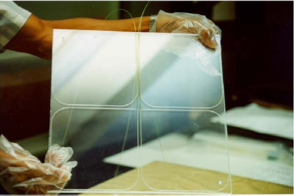
\includegraphics[width=\textwidth]{Figures/kuensken/hoTile.png}
\caption{Scintillator with the wavelength shifting fibers in sigma shape. Image from \cite{hoDesign}.}
\label{kuenskenScintWithFiber}
\end{minipage}
\hspace{1cm}
\begin{minipage}[t]{0.435\textwidth}

\end{minipage}
\end{figure}
From the wavelength shifting fibers the light is coupled into clear fibers to guide the light towards the photo-sensors. The tile's geometry is designed to match the towers of the HCAL in the barrel region which gives a tile size of 0.087$\times$0.087 in eta and phi. The scintillators are placed behind the solenoid in front of the first layer of the iron return yoke. While the rings $\pm$1 and $\pm$2 have only one layer of scintillator, ring 0 has a second layer of scintillator behind the iron yoke. This leads to specialties when bringing the light guiding fibers onto the photo-detectors, as is described in \ref{kuenskenHardwareDesign}.\\
With the upgrade of the photon sensors to SiPMs it is now subject to studies in how far HO has capabilities of detecting muons as MIPs\footnote{{\bf M}inimum {\bf I}onizing {\bf P}article} and providing a discrimination between MIP signals and leaking jets. The muon identification capability may be a key feature when thinking of providing an additional muon tag to the muon trigger system with the help of HO. A more thorough description of HO can be found in \cite{hcalTDR} and \cite{hoDesign}, information on the SiPM upgrade is available in \cite{beniCalor}.